% chap08 - Ordinary differential equations
% Last edited:

\chapter{Ordinary differential equations}

\section{A Note on Syntax}

Up until now, if you have followed the syntax that I've been using, especially
the guidelines that were layed out in Section~\ref{style1}, the code you've
written has been compatible with MATLAB. This means that someone who is
creating models in MATLAB can run your code and get the same results. In
general, Octave and MATLAB share vary similar syntax and function names.

However, starting with this chapter, we are going to introduce functions that
aren't compatible with MATLAB. Most of the syntax will be similar, so it won't
be difficult to modify your
code so it works with MATLAB. Nevertheless, don't expect the code you are about
to write to work with any program besides Octave. You will get many strange
errors if you try running it in MATLAB or any other scientific computing
program.

\section{Differential equations}

A {\bf differential equation} (DE) is an equation that describes the
derivatives of an unknown function. ``Solving a DE'' means finding a
function whose derivatives satisfy the equation.

For example, when bacteria grow in particularly bacteria-friendly
conditions, the rate of growth at any point in time is proportional to
the current population. What we might like to know is the population
as a function of time. Toward that end, let's define $f$ to be a
function that maps from time, $t$, to population $y$. We don't
know what it is, but we can write a differential equation
that describes it:

\[ \frac{df}{dt} = a f \]

where $a$ is a constant that characterizes how quickly the population
increases.

Notice that both sides of the equation are functions. To say that
two functions are equal is to say that their values are equal at
all times. In other words:

\[ \forall t: \frac{df}{dt}(t) = a f(t) \]

This is an {\bf ordinary} differential equation (ODE) because all the
derivatives involved are taken with respect to the
same variable. If the equation related derivatives with respect to
different variables (partial derivatives), it would be a {\bf partial}
differential equation.

This equation is {\bf first order} because it involves only first
derivatives. If it involved second derivatives, it would be second order,
and so on.

This equation is {\bf linear} because each term involves $t$, $f$ or
$df/dt$ raised to the first power; if any of the terms involved
products or powers of $t$, $f$ and $df/dt$ it would be
nonlinear.

Linear, first order ODEs can be solved analytically; that is, we
can express the solution as a function of $t$.
This particular ODE has an infinite number of solutions, but
they all have this form:

\[ t \to b e^{at} \]

For any value of $b$, this function satisfies the ODE. If you don't
believe me, take its derivative and check.

If we know the population of bacteria at a particular point in time,
we can use that additional information to determine which of the
infinite solutions is the (unique) one that describes a particular
population over time.

For example, if we know that $f(0) = 5$ billion cells, then we
can write

\[ f(0) = 5 = b e^{a 0} \]

and solve for $b$, which is 5. That determines what we wanted
to know:

\[ f : t \to 5 e^{at} \]

The extra bit of information that determines $b$ is called
the {\bf initial condition} (although it isn't always specified
at $t=0$).

Unfortunately, most interesting physical systems are described by
nonlinear DEs, most of which can't be solved analytically. The
alternative is to solve them numerically.


\section{Euler's method}

The simplest numerical method for ODEs is Euler's method. Here's a
test to see if you are as smart as Euler. Let's say that you
arrive at time $t$ and measure the current population, $y$, and
the rate of change, $r$. What do you think the population will
be after some period of time $h$ has elapsed?

If you said $y + r h$, congratulations! You just invented
Euler's method (but you're still not as smart as Euler).

This estimate is based on the assumption that $r$ is constant, but
in general it's not, so we only expect the estimate to be good if
$r$ changes slowly and $h$ is small.

But let's assume (for now) that the ODE we are interested in can
be written so that

\[ \forall t,y: \frac{df}{dt}(t) = g(t, y) \]

where $y=f(t)$ and $g$ is some function that maps $(t, y)$ onto $r$;
that is, given the time and current population, it computes the rate
of change. Then we can advance from one point in time to the
next using these equations:

\begin{eqnarray}
\label{euler1}
T_{n+1} = T_n + h       \\
\label{euler2}
F_{n+1} = F_n + g(t,y) h
\end{eqnarray}

where $T$ is a sequence of times where we estimate the value
of $f$, and $F$ is the sequence of estimates. For each
index $i$, $F_i$ is an estimate of $f(T_i)$.
The interval $h$ is called the {\bf time step}.

Assuming that we start at $t=0$ and we have an initial condition $f(0)
= y_0$ (where $y_0$ denotes a particular, known value), we would set
$T_1 = 0$ and $F_1 = y_0$, and then use \autoref{euler1} and \autoref{euler2}
% TODO: find a good way to do this reference
to
compute values of $T_i$ and $F_i$ until $T_i$ 
gets to the value of $t$ we are interested in.

If the rate doesn't change too fast and the time step isn't
too big, Euler's method is accurate enough for most purposes. One
way to check is to run it once with time step $h$ and then run it
again with time step $h/2$. If the results are the same, they are
probably accurate; otherwise, cut the time step again.

Euler's method is {\bf first order}, which means that each time you
cut the time step in half, you expect the estimation error to drop by
half. With a second-order method, you expect the error to drop by a
factor of 4; third-order drops by 8, etc. The price of higher order
methods is that they have to evaluate $g$ more times per time step.


\section{Another note on notation}

There's a lot of math notation in this chapter, and some of it is
non-standard, so I want to pause to review what we have so far.
Here are the variables, their meanings, and their types:

\begin{tabular}{|l|l|l|}
\hline
Name   & Meaning       & Type \\
\hline \hline
$f$   & The unknown function specified,  & function $t \to y$ \\
    & implicitly, by an ODE.       &  \\\hline

$df/dt$ & The first time derivative of $f$ & function $t \to r$ \\ \hline

$f_t$ & Alternative notation for the  & function $t \to r$ \\ 
    & first time derivative of $f$  & \\ \hline


$g$   & A ``rate function,'' derived from   & \\
    & the ODE, that computes rate of   & function $t, y \to r$ \\
    & change for any $t$, $y$.      &  \\\hline

$t$   & time      & scalar variable \\\hline
$y$   & population      & scalar variable \\\hline
$r$   & rate of change      & scalar variable \\\hline

$h$   & time step      & scalar constant \\\hline
$T$   & a sequence of times, $t$, where  & sequence \\
       & we estimate $f(t)$  &      \\\hline
$F$   & a sequence of estimates for $f(t)$ & sequence \\
\hline
\end{tabular}

So $f$ is a function that computes the population as a function of
time, $f(t)$ is the function evaluated at a particular time, and if we
assign $f(t)$ to a variable, we usually call that variable $y$.
Similarly, $g$ is a ``rate function'' that computes the rate of change as a
function of time and population. If we assign $g(t,y)$ to a variable,
we call it $r$.

$df/dt$ is the most common notation for the first derivative of $f$,
but I have never liked it because it looks like a fraction. I
prefer $f_t$, which has the benefit of looking like a function.

It is easy to get $f_t$ confused with $g$, but notice that they are
not even the same type. $g$ is more general: it can compute the rate
of change for any (hypothetical) population at any time; $f_t$
is more specific: it is the actual rate of change at time $t$, given
that the population is $f(t)$.

\section{{\tt lsode}}
\label{lsode}

Euler's method is an example of a {\bf fixed-step} differential equation solver.
It is a fixed-step solver because the time step is pre-determined and constant.
In other words, all
points that the DE solver calculates the function at will be equally
spaced. The alternative to a fixed-step solver is a {\bf variable-step} solver,
which -- like the name implies -- has a step size that changes as the function
value changes. We will examine some variable-step solvers in another section.
Right now we will learn how to use Octave's built-in fixed-step solver, {\tt
lsode}.

You could take time to write out a function for Euler's method, but using
{\tt lsode} is a much better choice. First of all, {\tt lsode} is already
written for you. There's no point writing your own fixed-step solver when
Octave already has one! More importantly, {\tt lsode} combines a number of
fixed-step solvers, many of which are much more powerful than
Euler's method. Using {\tt lsode} will make your code faster and more accurate.

To use {\tt lsode}, you will first have to write a Octave function
that evaluates $g$ as a function of
$t$ and $y$. As an example, suppose that the rate of population growth for rats
depends on the current population, $y$, and the availability of food,
which varies over the course of the year.
The governing equation might be something like

\[ f_t = a f \left[1 + \sin (\omega t) \right] \]
%
where $a$ is
a {\bf parameter}\footnote{A parameter is a value that appears
in a model to quantify some physical aspect of the scenario being
modeled. For example, in Exercise~\ref{duck} we used parameters
{\tt rho} and {\tt r} to quantify the density and radius of a
duck. Parameters are often constants, but in some models they
might vary in time.} 
that characterizes the reproductive rate, and
$\omega$ is the frequency of a periodic function that characterizes
the effect of varying food supply on reproduction.

This is an equation that specifies a relationship between a
function and its derivative. In order to estimate values of
$f$ numerically, we have to transform it into a rate function.
The first step is to write the equation more explicitly; to
say that two function are equal means that they are equal
all all times. In other words

\[ \forall t: f_t(t) = a f(t) \left[1 + \sin (\omega t) \right] \]
%
where $t$ is time in days. The next step is to introduce a variable,
$y$, as another name for $f(t)$

\[ \forall t: f_t(t) = a y \left[1 + \sin (\omega t) \right] \]

This equation means that if we are given $t$ and $y$, we can
compute $f_t(t)$, which is the slope, or rate of change, of $f$.
The last step is to express that computation as a function called
$g$:

\[ g : y, t \to a y \left[1 + \sin (\omega t) \right] \]

We have now written out the differential equation as a function, which we
can use with {\tt lsode} to estimate values of $f$. Here's
what the function looks like using the values $a = 0.01$
and $\omega = 2 \pi/365$ (one cycle per year):

\begin{verbatim}
function res = rats(y, t)
  a = 0.01;
  omega = 2 * pi / 365;
  res = a * y * (1 + sin(omega * t));
end
\end{verbatim}

You can test this function from the Command Window by calling it with
different values of {\tt t} and {\tt y}; the result is the rate of
change (in units of rats per day):

\begin{verbatim}
octave:1> r = rats(2, 0)
r = 0.020000
\end{verbatim}

So if there are two rats on January 1, we expect them to reproduce
at a rate that would produce 2 more rats per hundred days. But
if we come back in April, the rate has almost doubled:

\begin{verbatim}
octave:2> r = rats(2, 120)
r = 0.037600
\end{verbatim}

Since the rate is constantly changing, it is not easy to predict
the future rat population, but that is exactly what {\tt ode45} does.
Here's how you would use it:

\begin{verbatim}
octave:3> T = 0:5:365;
octave:4> Y = lsode(@rats, 2, T);
\end{verbatim}

With the first command, we are creating a vector for all the times that we want
to
find values of $f$ at. In this example, we want to know the rat population every
5 days for an entire year. Another way of saying this: we want our ODE solver
to find the population for an entire year with a step-size of 5 days.

In the second command, we are telling Octave to find a value for $f(t)$ at every
point in time that we specified in the first command. The first argument is a
handle for the function that
computes $g$. The second argument is the initial population, $f(0) = 2$. The
third argument is the vector containing the time values specified in the first
command.

You now know the rat population at every point during the year! To see what
this function looks like, plot the results.

\begin{verbatim}
octave:5> plot(T, Y, 'o-')
\end{verbatim}

Your plot should look something like this:

\beforefig \centerline{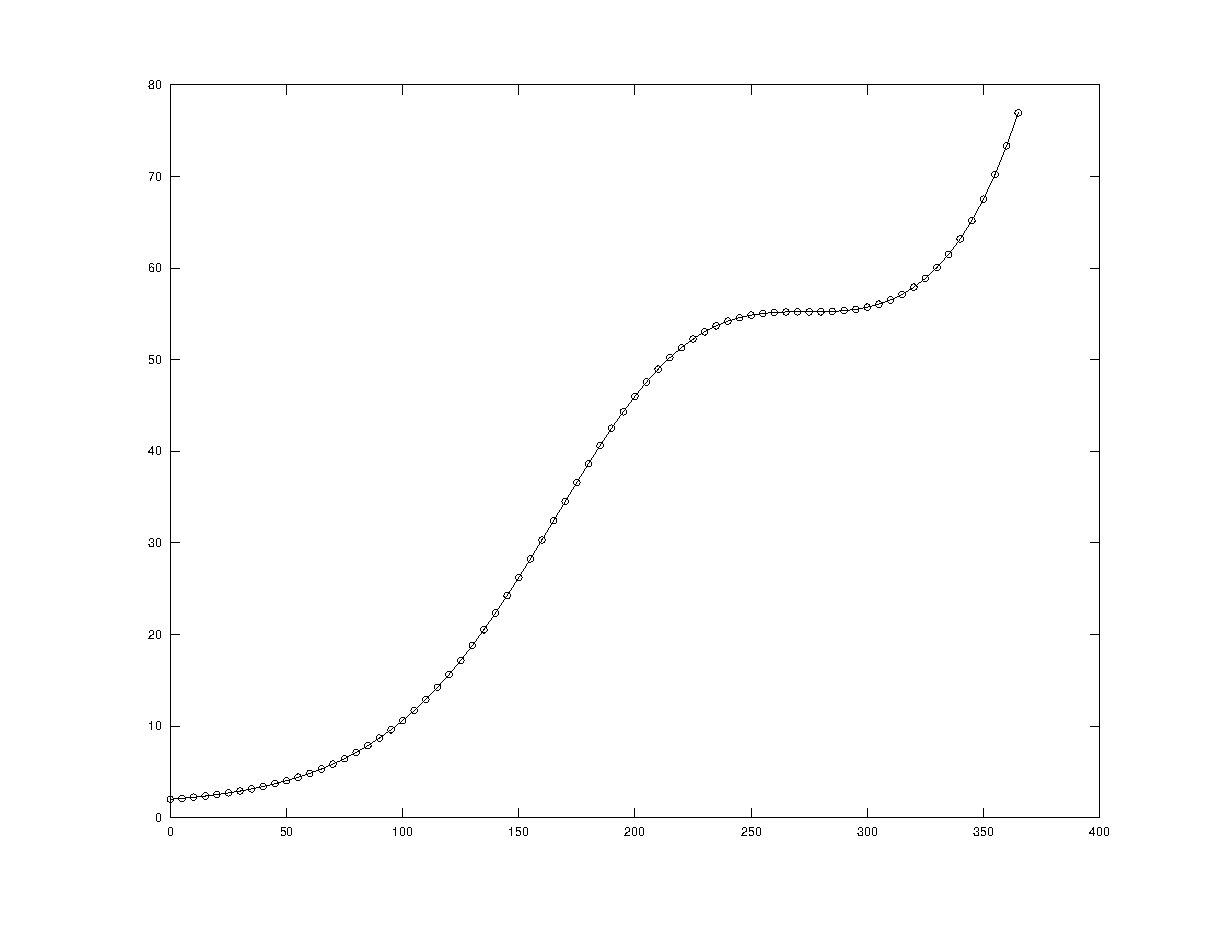
\includegraphics[height=2in]{figs/rats.eps}}

The x-axis shows time from 0 to 365 days; the y-axis shows the rat
population, which starts at 2 and grows to almost 80. The rate
of growth is slow in the winter and summer, and faster in the
spring and fall, but it also accelerates as the population grows.

%%% STOPPED HERE %%%

\section{{\tt ode45}}
\label{ode45}



%TODO: fix this

A limitation of fixed-step solvers is that the time step is constant from
one iteration to the next. But some parts of the solution are
harder to estimate than others; if the time step is small enough to
get the hard parts right, it is doing more work than necessary on the
easy parts. The ideal solution is to adjust the time step as you go
along. Methods that do that are called {\bf adaptive}, and one of the
best adaptive methods is the Dormand-Prince pair of Runge-Kutta
formulas. Fortunately, you don't have to know what that means,
because the nice people at Mathworks have implemented it in a function
called {\tt ode45}. The {\tt ode} stands for ``ordinary differential
equation [solver];'' the 45 indicates that it uses a combination of
4th and 5th order formulas.

%%%

When you call {\tt ode45} without assigning the result to a variable,
Octave displays the result in a figure:

\section{Multiple output variables}
\label{rats}

{\tt ode45} is one of many Octave functions that return more
than one output variable. The syntax for calling it and saving
the results is

\begin{verbatim}
octave:1> [T, Y] = ode45(@rats, [0, 365], 2);
\end{verbatim}

The first return value is assigned to {\tt T}; the second is assigned
to {\tt Y}. Each element of {\tt T} is a time,
$t$, where {\tt ode45} estimated the population; each element of {\tt
Y} is an estimate of $f(t)$.

If you assign the output values to variables,
{\tt ode45} doesn't draw the figure;
you have to do it yourself:

\begin{verbatim}
octave:1> plot(T, Y, 'bo-')
\end{verbatim}

If you plot the elements of {\tt T}, you'll see that the
space between the points is not quite even. They are closer
together at the beginning of the interval and farther apart at the end.

To see the population at the end of the year, you can display the
last element from each vector:

\begin{verbatim}
octave:1> [T(end), Y(end)]

ans = 365.0000  76.9530
\end{verbatim}

{\tt end} is a special word in Octave; when it appears as an index,
it means ``the index of the last element.'' You can use it in an
expression, so {\tt Y(end-1)} is the second-to-last element of
{\tt Y}.

How much does the final population change if you double the initial
population? How much does it change if you double the interval
to two years? How much does it change if you double the value
of $a$?


\section{Analytic or numerical?}

When you solve an ODE analytically, the result is a function, $f$,
that allows you to compute the population, $f(t)$, for any value of
$t$. When you solve an ODE numerically, you get two vectors. You can
think of these vectors as a discrete approximation of the continuous
function $f$: ``discrete'' because it is only defined for certain
values of $t$, and ``approximate'' because each value $F_i$
is only an estimate of the true value $f(t)$.

So those are the limitations of numerical solutions. The primary
advantage is that you can compute numerical solutions to ODEs that
don't have analytic solutions, which is the vast majority
of nonlinear ODEs.

If you are curious to know more about how {\tt ode45} works, you
can modify {\tt rats} to display the points, $(t, y)$, where
{\tt ode45} evaluates $g$. Here is a simple version:

\begin{verbatim}
function res = rats(t, y)
  plot(t, y, 'bo')
  a = 0.01;
  omega = 2 * pi / 365;
  res = a * y * (1 + sin(omega * t));
end
\end{verbatim}

Each time {\tt rats} is called, it plots one data point; in order
to see all of the data points, you have to use {\tt hold on}.

\begin{verbatim}
octave:1> clf; hold on
octave:1> [T, Y] = ode45(@rats, [0, 10], 2);
\end{verbatim}

This figure shows part of the output, zoomed
in on the range from Day 100 to 170:

\beforefig \centerline{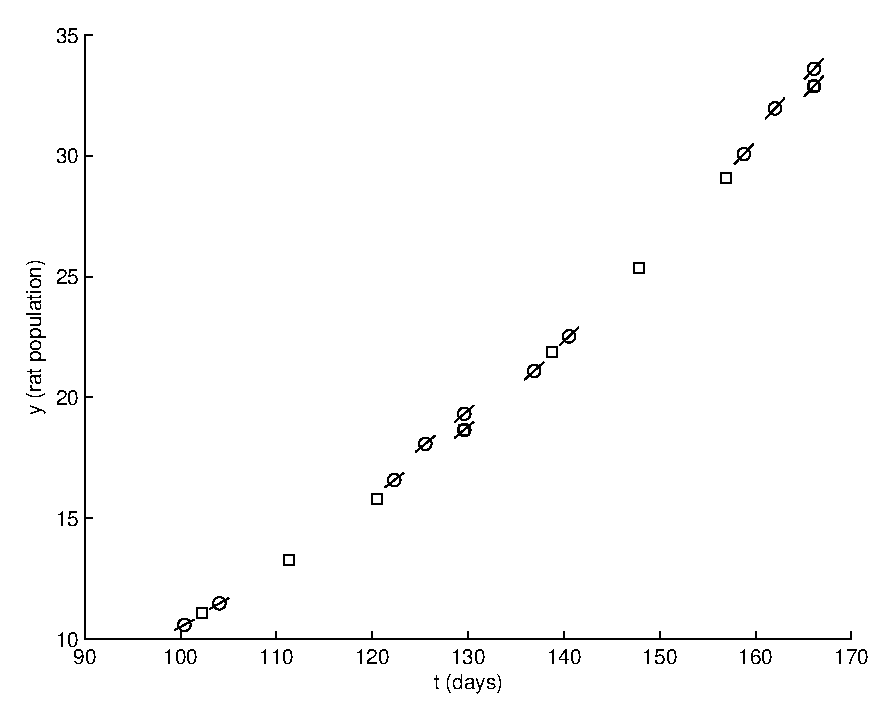
\includegraphics[height=2in]{figs/ode45.eps}}

The circles show the points where {\tt ode45} called {\tt rats}.
The lines through the circles show the slope (rate of change) calculated
at each point. The rectangles show the locations of the estimates
$(T_i, F_i)$. Notice that {\tt ode45} typically evaluates
$g$ several times for each estimate. This allows it to improve the
estimates, for one thing, but also to detect places where the errors
are increasing so it can decrease the time step (or the other
way around).


\section{What can go wrong?}

Don't forget the {\tt @} on the function handle.
If you leave it out, Octave treats the first argument as a function
call, and calls {\tt rats} without providing arguments.

\begin{verbatim}
octave:1> ode45(rats, [0,365], 2)
??? Input argument "y" is undefined.

Error in ==> rats at 4
  res = a * y * (1 + sin(omega * t));
\end{verbatim}

Again, the error message is confusing, because it looks like the problem
is in {\tt rats}. You've been warned!

Also, remember that the function you write will be called by
{\tt ode45}, which means it has to have the signature {\tt ode45}
expects: it should take two input variables, {\tt t} and {\tt y},
in that order, and return one output variable, {\tt r}.

If you are working with a rate function like this:

\[ g : t, y \to a y \]

You might be tempted to write this:

\begin{verbatim}
function res = rate_func(y)    % WRONG
  a = 0.1
  res = a * y
end
\end{verbatim}

But that would be wrong. So very wrong. Why? Because
when {\tt ode45} calls {\tt rate\_func}, it provides two arguments.
If you only take one input variable, you'll get an error. So
you have to write a function that takes {\tt t} as an input
variable, even if you don't use it.

\begin{verbatim}
function res = rate_func(t, y)   % RIGHT
  a = 0.1
  res = a * y
end
\end{verbatim}

Another common error is to write a function that doesn't make
an assignment to the output variable. If you write something
like this:

\begin{verbatim}
function res = rats(t, y)
  a = 0.01;
  omega = 2 * pi / 365;
  r = a * y * (1 + sin(omega * t))  % WRONG
end
\end{verbatim}

And then call it from {\tt ode45}, you get

\begin{verbatim}
octave:1> ode45(@rats, [0,365], 2)
??? Output argument "res" (and maybe others) not assigned during 
call to "/home/downey/rats.m (rats)".

Error in ==> rats at 2
  a = 0.01;

Error in ==> funfun/private/odearguments at 110
f0 = feval(ode,t0,y0,args{:});  % ODE15I sets args{1} to yp0.

Error in ==> ode45 at 173
[neq, tspan, ntspan, next, t0, tfinal, tdir, y0, f0, odeArgs, 
odeFcn, ...
\end{verbatim}

This might be a scary message, but if you read the first line
and ignore the rest, you'll get the idea.

Yet another mistake that people make with {\tt ode45} is leaving
out the brackets on the second argument. In that case, Octave
thinks there are four arguments, and you get

\begin{verbatim}
octave:1> ode45(@rats, 0, 365, 2)
??? Error using ==> funfun/private/odearguments
When the first argument to ode45 is a function handle, the 
tspan argument must have at least two elements.

Error in ==> ode45 at 173
[neq, tspan, ntspan, next, t0, tfinal, tdir, y0, f0, odeArgs, 
odeFcn, ...
\end{verbatim}

Again, if you read the first line, you should be able to figure
out the problem ({\tt tspan} stands for ``time span'', which we
have been calling the interval).


\section{Stiffness}

There is yet another problem you might encounter, but if it makes you
feel better, it might not be your fault: the problem you are trying to
solve might be {\bf stiff}\footnote{The following discussion is based
partly on an article from Mathworks available at
\url{
http://www.mathworks.com/company/newsletters/news_notes/clevescorner/may03_cleve
.html}}.

I won't give a technical explanation of stiffness here, except
to say that for some problems (over some intervals with some initial
conditions) the time step needed to control the error is very small,
which means that the computation takes a long time. Here's one
example:

\[ f_t = f^2 - f^3 \]

If you solve this ODE with the initial condition $f(0) = \delta$ over
the interval from 0 to $2/\delta$, with $\delta = 0.01$, you should
see something like this:

\beforefig \centerline{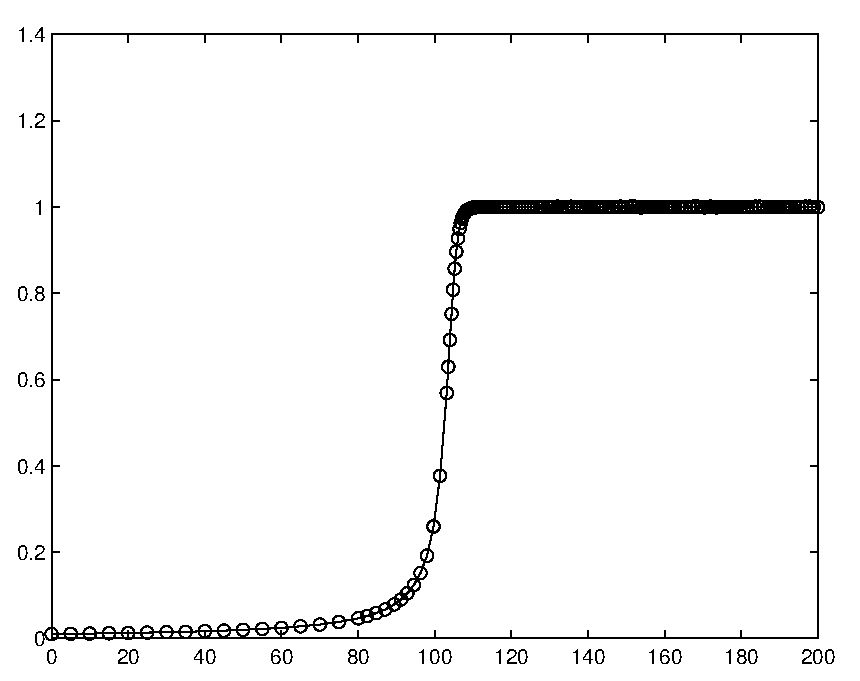
\includegraphics[height=2in]{figs/stiff.eps}}

After the transition from 0 to 1, the time step is very small and the
computation goes slowly. For smaller values of $\delta$, the
situation is even worse.

In this case, the problem is easy to fix: instead of {\tt ode45} you can
use {\tt ode23s}, an ODE solver that tends to perform well on stiff
problems (that's what the ``s'' stands for).

In general, if you find that {\tt ode45} is taking a long time, you
might want to try one of the stiff solvers. It won't always solve
the problem, but if the problem is stiffness, the improvement can
be striking.

\begin{ex}
Write a rate function for this ODE and use
{\tt ode45} to solve it with the given initial condition and interval.
Start with $\delta = 0.1$ and decrease it by multiples of 10. If
you get tired of waiting for a computation to complete, you can 
press the Stop button in the Figure window or press Control-C in
the Command Window.

Now replace {\tt ode45} with {\tt ode23s} and try again!
\end{ex}



\section{Glossary}

\begin{description}

\item[differential equation (DE):] An equation that relates the
derivatives of an unknown function.

\item[ordinary DE:] A DE in which all derivatives are taken with
respect to the same variable.

\item[partial DE:] A DE that includes derivatives with respect to
more than one variable

\item[first order (ODE):] A DE that includes only first derivatives.

\item[linear:] A DE that includes no products or powers of the
function and its derivatives.

\item[time step:] The interval in time between successive estimates
in the numerical solution of a DE.

\item[first order (numerical method):] A method whose error is expected
to halve when the time step is halved.

\item[fixed-step (solver):] An ODE solver that uses a constant
time step.

\item[variable-step (solver):] An ODE solver that has a time-step that changes
as the function value changes.

\item[adaptive:] A method that adjusts the time step to control error.

\item[stiffness:] A characteristic of some ODEs that makes some ODE
solvers run slowly (or generate bad estimates). Some ODE solvers,
like {\tt ode23s}, are designed to work on stiff problems.

\item[parameter:] A value that appears in a model to quantify some
physical aspect of the scenario being modeled.

\end{description}

\section{Exercises}

\newcommand{\degree}{\ensuremath{^\circ}}

\begin{ex}
Suppose that you are given an 8 ounce cup of coffee at 90 \degree C and
a 1 ounce container of cream at room temperature, which is 20 \degree C.
You have learned from bitter experience that the hottest coffee you
can drink comfortably is 60 \degree C.

Assuming that you take cream in your coffee, and that you would like
to start drinking as soon as possible, are you better off adding
the cream immediately or waiting? And if you should wait, then how
long?

To answer this question, you will have to model the cooling process
of a hot liquid in air. Hot coffee transfers heat to the environment
by conduction, radiation, and evaporative cooling. Quantifying these
effects individually would be challenging and unnecessary to answer
the question as posed.

As a simplification, we can use Newton's Law of
Cooling\footnote{\url{http://en.wikipedia.org/wiki/Heat_conduction}}:

\[ f_t = -r (f - e) \]
%
where $f$ is the temperature of the coffee as a function of time and
$f_t$ is its time derivative; $e$ is the temperature of the
environment, which is a constant in this case, and $r$ is a parameter
(also constant) that characterizes the rate of heat transfer.

It would be easy to estimate $r$ for a given coffee cup by making
a few measurements over time. Let's assume that that has been
done and $r$ has been found to be $0.001$ in units of inverse
seconds, $1/s$.

\begin{itemize}

\item Using mathematical notation, write the rate function, $g$,
as a function of $y$, where $y$ is the temperature of the
coffee at a particular point in time.

\item Create an M-file named {\tt coffee} and write a function
called {\tt coffee} that takes no input variables and returns no
output value. Put a simple statement like {\tt x=5} in the body
of the function and invoke {\tt coffee()} from the Command Window.

\item Add a function called
{\tt rate\_func} that takes {\tt t} and {\tt y} and computes
$g(t,y)$. Notice that in this case $g$ does not actually
depend on $t$; nevertheless, your function has to take $t$ as
the first input argument in order to work with {\tt ode45}.

Test your function by adding a line like {\tt rate\_func(0,90)}
to {\tt coffee}, the call {\tt coffee} from the Command Window.

\item Once you get {\tt rate\_func(0,90)} working, modify
{\tt coffee} to use {\tt ode45} to compute the temperature
of the coffee (ignoring the cream) for 60 minutes. Confirm that
the coffee cools quickly at first, then more slowly, and reaches
room temperature (approximately) after about an hour.

\item Write a function called {\tt mix\_func} that computes
the final temperature of a mixture of two liquids. It should
take the volumes and temperatures of the liquids as parameters.

In general, the final temperature of a mixture depends on the specific
heat of the two
substances\footnote{\url{http://en.wikipedia.org/wiki/Heat_capacity}}.
But if we make the simplifying assumption that coffee and cream
have the same density and specific heat, then the final temperature is
$(v_1 y_1 + v_2 y_2) / (v_1 + v_2)$, where $v_1$ and $v_2$ are
the volumes of the liquids, and $y_1$ and $y_2$ are their
temperatures.

Add code to {\tt coffee} to test {\tt mix\_func}.

\item Use {\tt mix\_func} and {\tt ode45} to compute the
time until the coffee is drinkable if you add the cream
immediately.

\item Modify {\tt coffee} so it takes an input variable $t$ that
determines how many seconds the coffee is allowed to cool before
adding the cream, and returns the temperature of the coffee
after mixing.

\item Use {\tt fzero} to find the time $t$ that causes the
temperature of the coffee after mixing to be 60 \degree C.

\item What do these results tell you about the answer to the original
question? Is the answer what you expected? What simplifying
assumptions does this answer depend on? Which of them do you think
has the biggest effect? Do you think it is big enough to affect the
outcome? Overall, how confident are you that this model can give
a definitive answer to this question? What might you do to improve
it?

\end{itemize}

\end{ex}
